\documentclass[11pt]{article}

\usepackage{setspace}
\usepackage[margin=1in]{geometry}

% Make table of contents look better
\usepackage{tabularx}
\usepackage{tocloft}
\renewcommand{\cftsecleader}{\cftdotfill{\cftdotsep}}

\usepackage{graphicx}
\usepackage{pdfpages}
\usepackage{hyperref}

% \usepackage[ngerman]{babel}
% \usepackage[T1]{fontenc}
% \usepackage[ansinew]{inputenc}
% \usepackage{lmodern}

% Times New Roman font
\usepackage{txfonts}

\begin{document}

\setlength{\parindent}{2em}

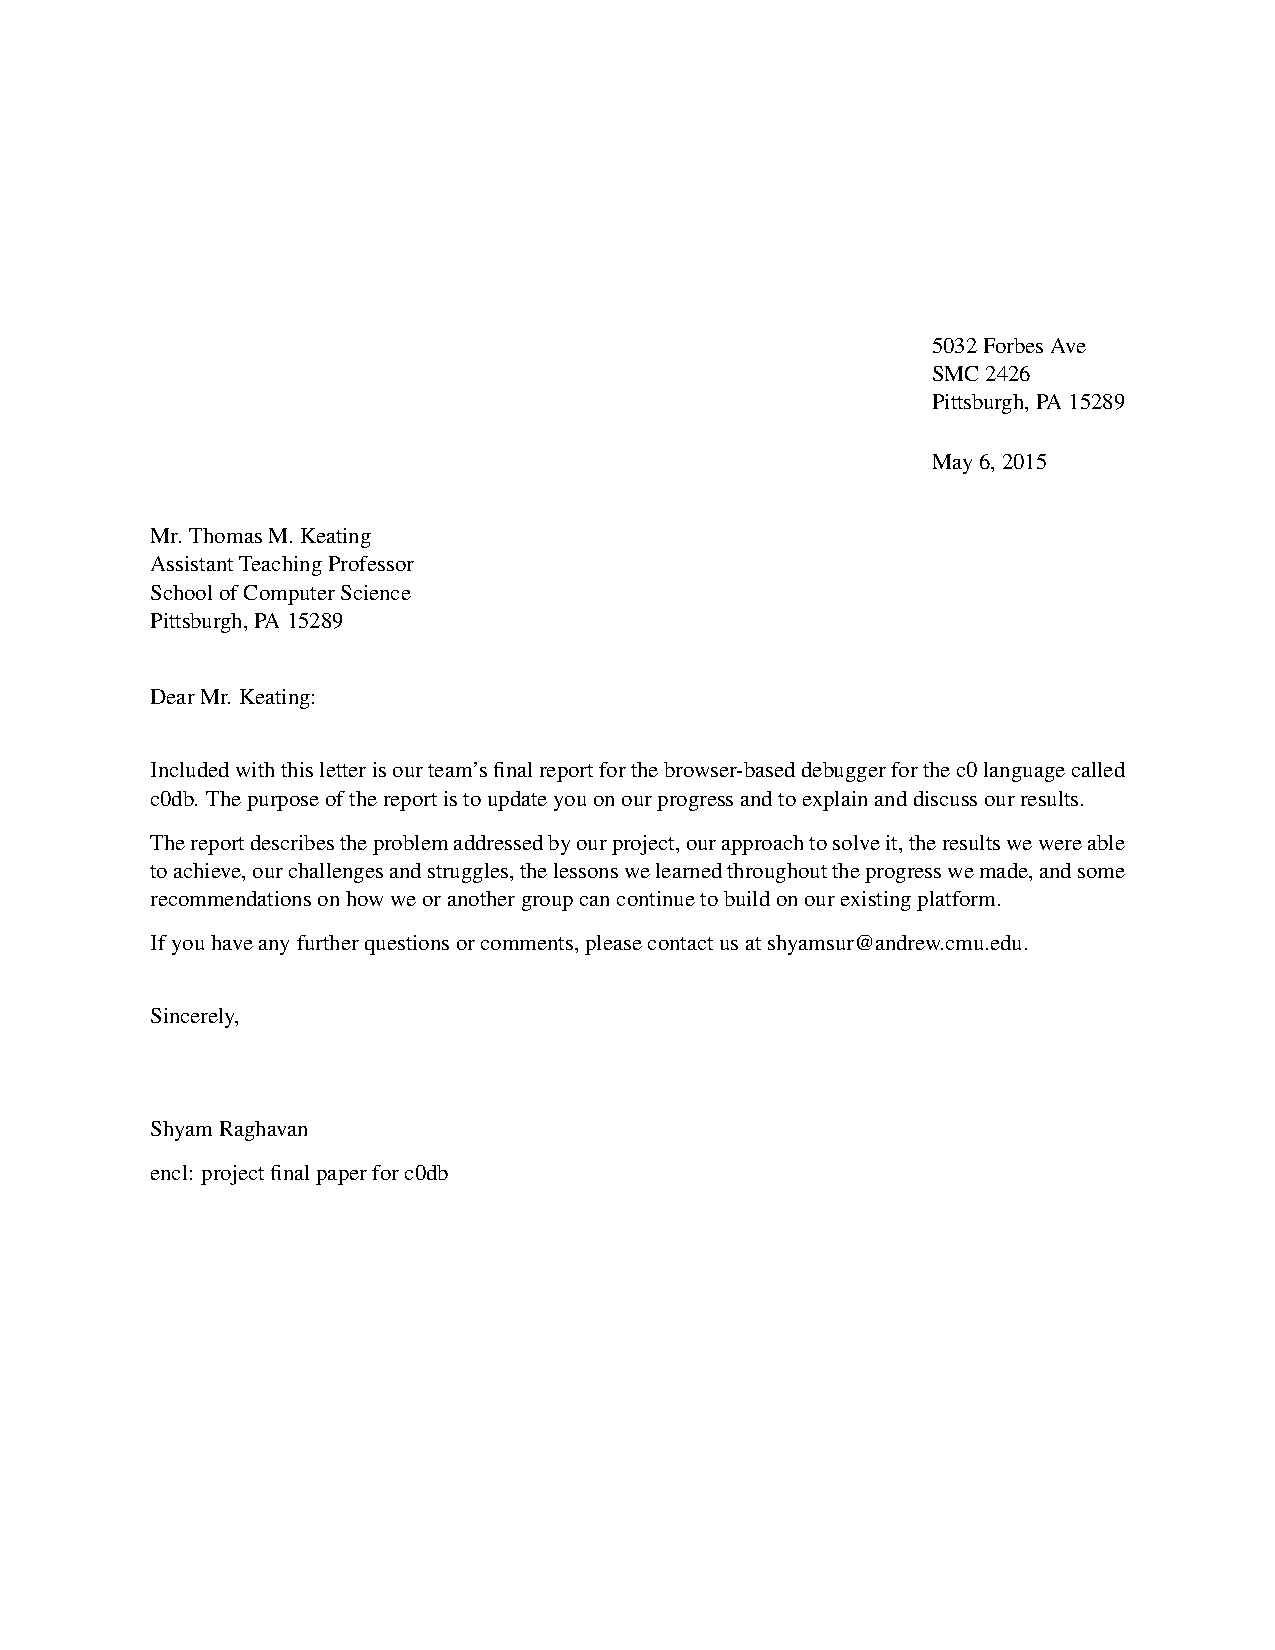
\includepdf[pages={1}]{letter.pdf}

\begin{titlepage}
\clearpage
\thispagestyle{empty}

\begin{center}
{\Huge Final Report}\\
\vspace{10 mm}
{\Huge The {\tt C0} Debugger}\\
\vspace{10 mm}

Submitted to\\
Mr. Thomas M. Keating\\
Assistant Teaching Professor\\
School of Computer Science\\
Pittsbugh, PA 15289

\vspace{10 mm}

Prepared by\\
{\bf Aaron Gutierrez}\\
{\bf Shyam Raghavan}\\
Mitchell Plamann\\
Suhaas Reddy

\vspace{10 mm}

School of Computer Science\\
Carnegie Mellon University\\
\today

\vspace{10 mm}

{\bf Abstract}
\end{center}
\par
This project is a proposal for C0 Debugger, a browser-based debugger for the
C0 programming language.
Students in Carnegie Mellon University's 15-122: Principles of Imperative
Computation and other classes learn to program in C0.
This project will allow students to better write C0 code by providing a
powerful and easy-to-use system for debugging their C0 programs.
This proposal goes over a detailed plan for how our team will create the C0 Debugger.
\end{titlepage}

\pagenumbering{roman}
\tableofcontents
\newpage

\pagenumbering{arabic}

\section{Introduction}

\section{Approach}

\section{Results}

\section{Discussion}

\section{Sources Cited}

\end{document}
